\documentclass[sigplan, screen, 10pt]{acmart}
\renewcommand\footnotetextcopyrightpermission[1]{}
\settopmatter{printfolios=false,printccs=false,printacmref=false}

\acmYear{2024}\copyrightyear{2024}
\acmConference[Brown CS1380'24]{Brown's Distributed Computing Systems}{Spring, 2024}{Providence, RI}
% \acmBooktitle{}
% \acmPrice{}
% \acmDOI{}
% \acmISBN{}

\usepackage{enumitem}
\usepackage{booktabs}
\usepackage{soul}
\usepackage{xspace}
\usepackage{color}
\usepackage{xcolor}
\usepackage{upquote}
\usepackage{listings}
\usepackage{amsmath}
\usepackage{wrapfig}
\usepackage{syntax}
\usepackage{caption}
\usepackage{picins}
\usepackage{minted}

\newcommand{\eg}{{\em e.g.}, }
\newcommand{\ie}{{\em i.e.}, }
\newcommand{\etc}{{\em etc.}\xspace}
\newcommand{\vs}{{\em vs.} }
\newcommand{\cf}[1]{(\emph{Cf}.\S\ref{#1})}
\newcommand{\sx}[1]{(\S\ref{#1})}
\newcommand{\sys}{{\scshape pSys}\xspace}

\renewcommand{\shortauthors}{J. S. Carberry}

\bibliographystyle{ACM-Reference-Format}

\usepackage{booktabs}
\usepackage{subcaption}

\title{CourseCluster: a distributed course registration system}

\author{Alex Lin}
\affiliation{Brown University}
\email{alex_lin@brown.edu}
\author{Ethan Williams}
\affiliation{Brown University}
\email{ethan_williams@brown.edu}
\author{Ben Bachmann}
\affiliation{Brown University}
\email{ben_bachmann@brown.edu}

\begin{document}

\begin{abstract}
  This paper presents the design, implementation, and evaluation of CourseCluster, a distributed and scalable course registration system developed for CS1380 at Brown University. CourseCluster is designed to manage large volumes of student and course data, ensuring scalability and data consistency across nodes. We deployed our system to Elastic Compute Cloud (EC2) instances on Amazon Web Services (AWS) to enhance performance and stability across multiple nodes, and connected the system to a simple interface.
\end{abstract}

\maketitle

% \pagestyle{plain}

\section{Introduction}

In an increasingly digitised world, effective online course registration systems are a centrepiece of the modern university experience. We present CourseCluster, a distributed system designed to handle the complexities of course registration at a university level. Our implementation consists of an architecture intended to support the querying of and registration for courses by students through a web interface.

Our distributed system is structured around two key datasets: our courses dataset contains a list of courses offered, including its title, course id, subject, description, and prerequisites. These were scraped from a website hosted by Brown University’s servers. Our students dataset contains a list of artificial student names, along with their semester level and a list of courses taken. The list of student names were randomly selected from a list of common first names \cite{babynames}. These datasets are each partitioned across a node group.

For simplicity, the system relies on a number of assumptions that are typical in academic settings, including the absence of enrolment limits for courses, and the immutability of the authoritative course and student lists. Additionally, while our system is not designed to handle node failures, we discuss the possibility for implementing a fault tolerant system in the future.

The client nodes orchestrate the registration processes. Once a student submits a registration, the client nodes ensure that the student has met the prerequisites and is not already registered for 5 courses. We implemented a locking mechanism to ensure atomicity of the registration operation. Similarly, when a student submits a search request, the client node is responsible for sending this requests to all the courses nodes, and aggregating the results. The search operation is implemented using a MapReduce \cite{mapreduce} framework, which generates the capability to scale to a large volume of concurrent searches without significant performances losses. 

We open our discussion in Section 2 with an example user workflow, and the functionality just outlined is described in detail in Section 3. Our system also enables users to search our course catalogue by keyword- Section 4 describes our implementation of an algorithm inspired by the PageRank algorithm implemented by Sergey Brin and Larry Page in 1998 at Google \cite{google}. We include the technical details of our implementation, some design considerations, as well as performance concerns. In Section 5, we discuss the deployment of our system to run on EC2 instances on AWS. We include details of the EC2 instances used, the types of nodes hosted on the AWS infrastructure, and the performance gains. In Section 6 we discuss our system’s performance against various metrics, including its ability to handle large volumes of concurrent requests, and its performance with increased numbers of nodes. Section 7 discusses the implications of our system, its limitations, and imagines some ways in which it could change the landscape of higher-level education. Finally, in Section 8, we discuss related work.

\section{Example}
\label{bg}

To illustrate the intended usage of our distributed course registration system, we consider a typical scenario where a student, Alice, seeks to register for courses at the beginning of a semester. The entire process occurs through our web interface.
\subsection{User Login}
First, Alice submits a login request by entering her student details into the provided text fields. Provided that she sends her unique student token as input, she will be logged in successfully and be able to register for courses for which she meets the prerequisites and is in the right semester to take.

\subsection{Dashboard Functionality and Course Search}
Suppose, then, that she is searching for a course on distributed systems. She will then send a search request, likely with the keywords 'distributed systems'. The client node responsible for handling Alice's request will then send this query to all the courses nodes, which are responsible for storing all the course data. These nodes perform a search based on the MapReduce \cite{mapreduce} framework, which efficiently processes large datasets by distributing the tasks across multiple nodes. This framework is designed to handle large volumes of course data and many student queries simultaneously, as the demands of large universities require.

\subsection{Aggregation and Display of Search Results}
Once the course nodes complete their respective searches, they send the results back to the client node. The client node then aggregates these results, and the result returned via the interface is a list of the courses that most closely match her query. Each result includes key information such as course title, description, and prerequisites.

\subsection{Course Registration Process}
Once Alice decides on a course, she uses the interface to register for that course, which initiates a register request. The system first checks whether Alice has already registered for the maximum allowed number of courses (five), and whether she meets all the prerequisites for the course. Assuming that these conditions are met, the client node communicates with both student and course nodes in order to lock the registration. This prevents any registration conflicts that could arise from multiple students attempting to register for the same course simultaneously. If the client node successfully obtains both locks, Alice is registered for her chosen course. The course node updates its records to include Alice as a registered student, and the student node updates Alice's records to reflect her enrolment in the new course.

\section{View and Control}
We designed our system to scale to a large number of nodes and concurrent requests. This section describes the details of how the system processes requests under the hood.

\begin{figure}[t]
  \centering
  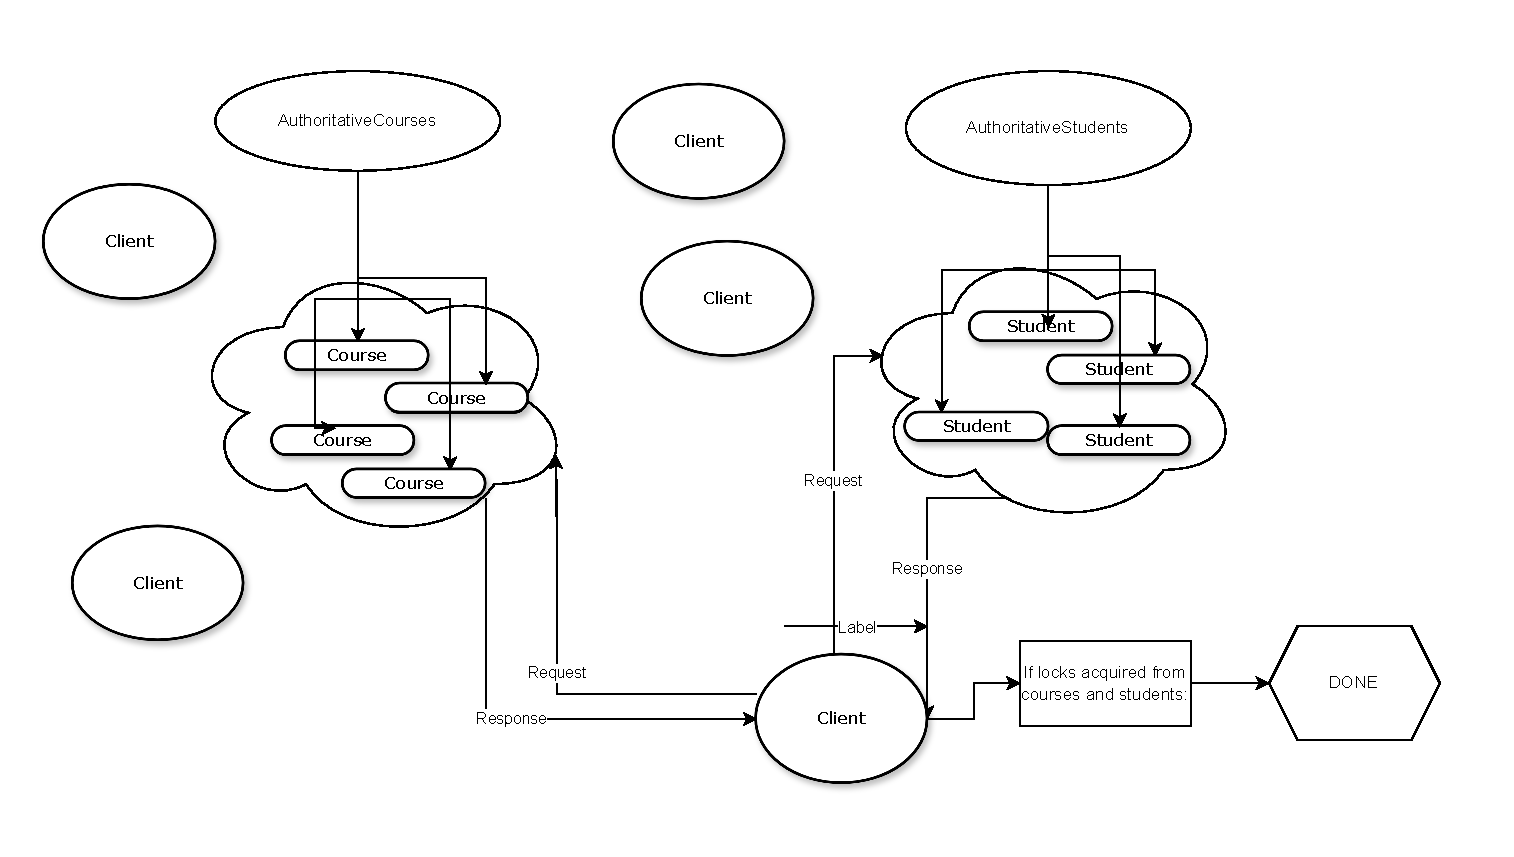
\includegraphics[width=0.49\textwidth]{./figs/overview.pdf}
  \caption{
    \textbf{CourseCluster architecture}
  }
  \vspace{-18pt}
  \label{fig:overview}
\end{figure}

\subsection{Coordinator Nodes}
We structured our implementation around two coordinator nodes, 'authoritativeCourses' and 'authoritativeStudents', which hold the authoritative data regarding courses and students respectively. For each of these coordinator nodes, we implemented 'list' and 'detail' services, which return a complete list of courses/students and details about a single course/student respectively.

\subsection{Client and Registration Nodes}
Users of our interface talk to a client node. In contrast to the authoritativeCourses and authoritativeStudent nodes, there may be many client nodes. This helps to distribute the load. Finally, there may be any number of 'students' and 'courses' nodes. These are equipped with lock and unlock services to ensure that the registration procedure either succeeds or has no effect, and with submit and listRegister services which submit and list all courses associated with a student or vice versa respectively.

\subsection{Scalability}
Course registration generally opens for large batches of students simultaneously. This leads to course registration requests being heavily clustered towards the hours following the opening of course registration. It is necessary to ensure that our system can scale to handle this sudden increase in requests. We discuss scalability in greater depth in Section 6.

\subsection{Fail-Safe Mechanism}
In addition, we prioritised a fail-safe system. If a registration operation fails, the system will enter a state as if that operation had not occurred. This ensures that at peak hours, an overloading of requests will not lead the system to break. Instead, the student may need to make several registration attempts before the request successfully goes through.

\subsection{Interface Design}
\begin{figure}[!htb]
  \centering
  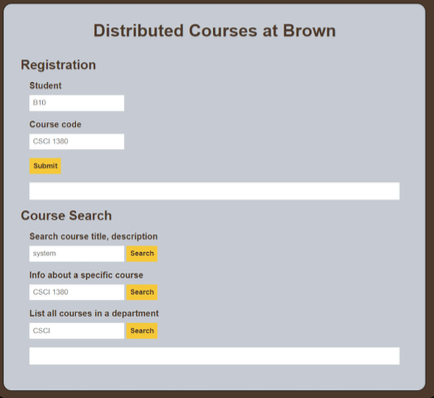
\includegraphics[width=0.49\textwidth]{./figs/webpage.png}
  \caption{
    \textbf{CourseCluster User Interface}
  }
  % \vspace{-18pt}
\end{figure}
We emphasised simplicity and intuitiveness in our design of the web interface. The course's entire functionality, including search, login, and registration, is contained within a single web page. We subdivided the page into two sections: 'Registration' and 'Course Search'. This keeps these two functionalities distinct, whilst ensuring that students can register simply by entering the correct information into two fields. In addition, our interface allows students to see the results of their most recent search under the 'Course Search' section, whilst simultaneously submitting a registration request. This dual functionality within a single web page prevents users from having to remember or write down the results of a past search in order to register for their chosen course.

\section{Search}
Given the large number of courses offered in a typical university, it is necessary to develop a sophisticated search algorithm in order to effectively be able to retrieve course that best match the user's wishes. To achieve this, we implemented an algorithm inspired by the PageRank algorithm \cite{google}, combined with indexing and data distribution techniques. This section describes the key features of our implementation.

\subsection{Adapting PageRank for Searching Course Catalogues}
The PageRank algorithm was first invented by Sergey Brin and Larry Page in 1998 to rank the importance of web pages based on their link structures, word frequencies, and inverse document frequencies. We have adapted their approach for our search endpoint within CourseCluster, enabling users to search by a text query, for a specific course, or by academic department.

\subsection{TF-IDF and Stemming}
We used the Term Frequency-Inverse Document Frequency (TF-IDF) metric in our system to improve the precision of our search results. This method allows us to rank pages with a greater frequency of the query term as more closely matching the intent behind the user's query, whilst also considering the frequency of the term in relation to other documents, in order to determine whether a term is important for a document in particular, or whether the term is a generally common word across all documents. Using stemming techniques, we reduced words to their base form, to allow for different grammatical forms of words with near-identical meaning.

\subsection{Indexing Courses}
We concatenate the course name and description, and run our search query against this index. When a query is received, the system matches it against this index.

\subsection{Consistent hashing}
We partitioned our datasets across two node groups: 'courses' to store course data, and 'students' to store student data. This ensures that the storage is evenly balanced across the nodes. We used a consistent hashing scheme to ensure that each shard of data gets mapped to the same node, ensuring that the overall state of the system is coherent between the nodes.

\subsection{Scalability}
Course lists at any modern university are generally published on a prespecified date. This leads to a substantial increase in the number of searches made in the hours that follow. We therefore designed our system to be able to handle a large number of request in as short a time as possible without breaking. We achieved this through the deployment of our system on cloud services, as described in Section 5.

\subsection{Design Considerations}
A key assumption of our system is that the course and students lists do not change. Our search algorithm therefore always operates against the same index. In order to account for incoming or outgoing students, for course addition or deletion, updating the course description, correcting a misspelt student name, and so on, we would need to devise a set of endpoints for adding, deleting, and updating these fields, and implement an appropriate mechanism to add the new student or course data to the correct shard, whilst ensuring that all nodes agree on the state of the system.

\section{Deployment}
We deployed eleven nodes- one authoritativeCourses, one authoritativeStudent, three Student, three Courses, and three Client- on Elastic Cloud Compute (EC2) instances on Amazon Web Services (AWS). We discuss performance gains due to our deployment in Section 6. We used EC2 Micro instances, since these are a cost-effective solution suited to low-traffic scenarios. In order to scale to larger numbers of students, we would consider using larger EC2 instances for our nodes.

\section{Evaluation}
Our system requires an authoritativeCourses and authoritativeStudent node, as well as at least one client node for the user to interact with. We tested our system with variable numbers of client, student, and course nodes and measured the relative performance across these different configurations.

\subsection{Registration Throughput}

\begin{figure}[!htb]
  \centering
  \includegraphics[width=0.49\textwidth]{./figs/registrationthroughput.pdf}
  \caption{
    \textbf{Registration Throughput}
  }
  % \vspace{-18pt}
\end{figure}

We measured the throughput of our registration system with one, two, and three client nodes. For each number of client nodes, we measured the throughput with one, two, and three (of each) course and student nodes. We found that additional client nodes substantially improved throughput, whereas increasing the number of student and course nodes had a minimal effect on throughput. Using three client nodes, the average number of registrations per second, measured across 1000 trials, was 260.

\subsection{Query Throughput}
\begin{figure}[!htb]
  \centering
  \includegraphics[width=0.49\textwidth]{./figs/querythroughput.pdf}
  \caption{
    \textbf{Query Throughput}
  }
  % \vspace{-18pt}
\end{figure}
We measured the throughput of our query system in similar fashion to our measurement of registration throughput. We found once again that increasing the number of client nodes substantially improved throughput, whereas we found no statistically significant effect of scaling up from one student and one course node to three student and three course nodes. For 3 client nodes, the average number of queries handled per second, measured across 100 trials, was 19.

\subsection{Registration Latency}
\begin{figure}[!htb]
  \centering
  \includegraphics[width=0.49\textwidth]{./figs/registrationlatency.pdf}
  \caption{
    \textbf{Registration Latency}
  }
\end{figure}
We measured the latency of our registration system over 1000 trials. Over 95 percent of our trials were processed within 30ms, with the majority being processed within 23ms. We experienced a few outliers that took over 100ms to process.

\subsection{Query Latency}
\begin{figure}[!htb]
  \centering
  \includegraphics[width=0.49\textwidth]{./figs/querylatency.pdf}
  \caption{
    \textbf{Query Latency}
  }
\end{figure}
We also measured the latency of our query system over 1000 trials. Results were more variable than for our registration system. The majority of queries were processed in under 100ms, though some took 200ms, and a few outliers took over 300ms.

\subsection{Benchmarks}
\begin{figure}[!htb]
  \centering
  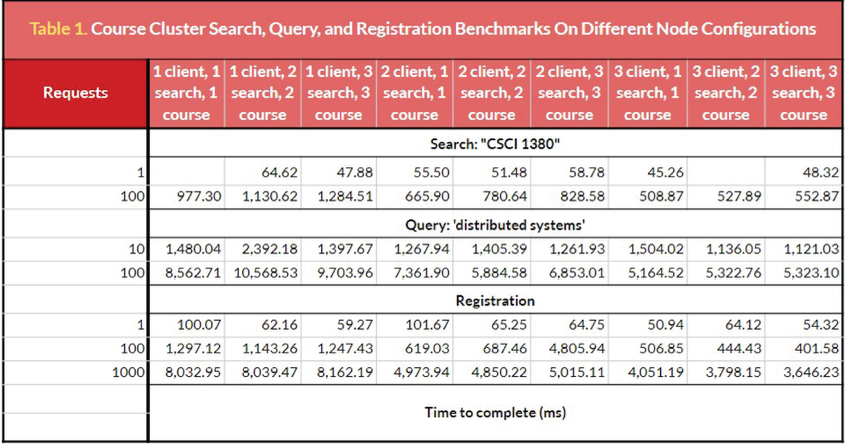
\includegraphics[width=0.49\textwidth]{./figs/nodeconfigurations.png}
  \caption{
    \textbf{Search, Query, and Registration Benchmarks}
  }
  % \vspace{-18pt}
\end{figure}
\begin{figure}[!htb]
  \centering
  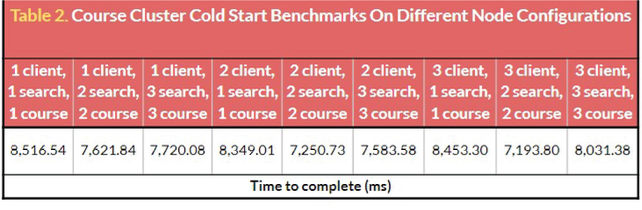
\includegraphics[width=0.49\textwidth]{./figs/coldstart.png}
  \caption{
    \textbf{Cold Start Benchmarks}
  }
  % \vspace{-18pt}
\end{figure}
Figures 5 and 6 display benchmarks for cold starting the system, as well as for the search, query, and registration operations. We find no statistically significant difference in the cold start time for different numbers of client nodes, suggesting that while distributing the load across additional nodes improves performance, there are additional overhead costs to introducing more client nodes. However, adding an extra student and course node tends to yield a moderate cold start performance improvement. For the benchmarks, we find substantial performance improvements associated with adding extra client nodes, across all three operations. In addition, we see that the time for the requests to complete scales faster than linearly with the number of requests, indicating that distributing our operations across multiple nodes enables our system to scale. While we do no not know the upper limit of the number of concurrent requests our system can handle, with three client nodes, our systems is able to register 1000 students within 4 seconds.

\section{Discussion}
Whilst CourseCluster is impressive as an end-to-end product, we recognise the potential for added features, broader applications, and other improvements. This section discusses some future directions for our distributed course registration system.

\subsection{Improved Search}
In future versions, we would add functionality to search based on multiple parameters. For example, one might search simultaneously by subject and a text query. This would help improve results. Consider the case where a student searches for the term 'CSCI1380'. Clearly in this case, the user wants to find the course in the CSCI department with ID 1380. However, if there is another course with the string 'CSCI1380' listed in its metadata, such as in its prerequisites, these could nevertheless appear first in the search results.

\subsection{Future of Education}
Before the internet became widespread, course registration at universities was generally done in person. Students would fill out paper forms and submit them to a registration office, often involving long queues and a large volume of error-prone work by representatives entering students' names in rosters. Our distributed course registration system increases the efficiency of these administrative processes within universities.

We also see the potential for a transformation of the nature of education more broadly, such that administrative processes would be made more efficient not just within universities but between them as well. Given improved search results, and improved scalability, one could imagine our system scaling to millions of nodes or more. This could enable the distribution of our course registration system amongst not just the nodes of a single university, but nodes from multiple different universities. This could be leveraged in a large, online university, where students from all over the world can register for courses offered at thousands of institutions. Prospective students would be able to filter by institution, subject, keywords, professor, time zone, and much more, to find a course that fits their wishes precisely. Such a system would have an orders of magnitude increase in the subjects available for people to study. Further, it would help match professors who teach more niche subjects and therefore struggle to find a large audience for their classes locally and therefore fail to get the course approved for teaching by the authorities.

\subsection{Machine Learning Integration}
Predictive analytics could be used to forecast course popularity and thus aid in the decision-making behind what courses are offered. It could also be used to improve the search experience for users. By storing a student's course history, an ML algorithm could be used to predict what courses a student is likely to be interested in, and push those courses up in the search results ranking. The course catalogue could thus be made to function like a recommendation system.

\subsection{Improved User Experience}
The web interface could be built out to include more sophisticated user flows, and other features. Future versions could include advanced search features, such as autocomplete suggestions based on a student's search history, as well as personalised recommendations based on a student's concentration and academic history. Future versions should also integrate two-factor authentication (2FA), and other protection for student data privacy. In addition, future versions could include a real-time notification system to inform students of academic deadlines, and other information relating to their studies.

\section{Related Work}
CourseCluster draws on seminal works from a variety of fields within and related to distributed systems. We studied Hamilton’s 2007 paper \cite{deploying} as we were making design choices and considering tradeoffs between scalability and performance. Brin and Page’s PageRank algorithm \cite{google} was the fundamental inspiration for our own search engine. Dean and Ghemawat’s work on the MapReduce framework \cite{mapreduce} laid the foundation for our data processing capabilities.

\section{Conclusion}

In this paper, we presented a distributed course registration system designed to handle the most important demands of a modern educational institution. Our system included functionality for course registration, as well as to search the course database by keyword. We demonstrated that the system could scale to handle a large number of concurrent requests and across dozens of nodes.

Some things we learned are:
\begin{enumerate}
  \item the importance of rigorous synchronisation and transaction protocols to ensure data consistency across nodes,
  \item the importance of effectively balancing performance and complexity depending on the use-case, and
  \item the complexity involved in building a search engine that consistently returns the results that the user is looking for.
\end{enumerate}

We have open-sourced our implementation. The full code can be found at this link: 
\url{https://github.com/EtomicBomb/} \\
\url{distributed-systems-final-project}


%% Bibliography
{\small
\bibliography{./bib}
}

\appendix

\section{Reflections}
\label{reflections}

% Roughly, how many hours did **the paper** take you to complete?

Hours for paper: <25>

\section{Using our System}
\label{using-apx}

Our system is available on the link \url{http://52.87.235.205/}
Note that due to cost limitations, we cannot run our EC2 instances indefinitely, so this link will no longer be available after a certain timeframe.

\end{document}